% !TEX program = pdflatex
% !BIB program = biber
\documentclass[11pt,
	a4paper,
	bibliography=totocnumbered,   % totoc
	captions=tableheading,
	headings=normal,
	parskip=half*,
	chapterentrydots=true,
	numbers=noenddot
	]{scrreprt}

% Define the number of the work here
\newcommand{\thesisNo}{4xxxxx}

% load packages
%scrhack, um @addtolists warnings zu unterdrücken, bei Paketen, die KOMA kennt (insbesondere listings)
\usepackage{scrhack}
\usepackage[T1]{fontenc}
\usepackage[utf8]{inputenc}
\usepackage[english]{babel}
\usepackage[scaled=1]{uarial} % set default font to arial
\renewcommand{\familydefault}{\sfdefault}
\usepackage{multirow}
\usepackage{float}
\usepackage{csquotes}

% enable hyperlinks in pdf documennt
\usepackage[hidelinks]{hyperref}
\usepackage[colorinlistoftodos]{todonotes}\reversemarginpar

%enable \gls
\usepackage[automake,nonumberlist,acronym,toc,nopostdot,nomain,numberedsection=autolabel]{glossaries}
\newglossary[slg]{symbolslist}{syi}{syg}{Symbols} % create add. symbolslist
\makeglossaries
% Displays unit in symbole list
\newglossarystyle{symbunitlong}{
	\setglossarystyle{long4col}
	\renewcommand*{\glossentry}[2]{
		\glstarget{##1}{\glossentryname{##1}} %
		& \glssymbol{##1}
		& \glossentrydesc{##1}  \tabularnewline
	}
}
\makeindex
\setacronymstyle{long-short}
\glsaddall

%% the following commands are needed for some matlab2tikz features
\usetikzlibrary{plotmarks}
\usetikzlibrary{arrows.meta}

\usepackage{graphicx}
\usepackage{tkz-euclide}
\usepackage{pgfplots}
\usepackage{tikzscale}
\pgfplotsset{
    every tick label/.append style = {/pgf/number format/assume math mode=true,font=\sffamily},
}
\pgfplotsset{max space between ticks=50}
\pgfplotsset{compat=newest}


%\usepackage{grffile}
\usepackage{amsmath}
\usepackage{listings}
\usepackage{rotating}
\usepackage{cleveref}
%\crefname{equation}{eq.}{eqs.}
%\Crefname{equation}{Eq.}{Eqs.}
\crefformat{equation}{Eq.~#2#1#3}
\Crefformat{equation}{Eq.~#2#1#3}
%\crefformat{subfigure}{Fig.~#2(#1)#3}
\crefname{table}{Fig.}{Figs.}
\crefname{figure}{Fig.}{Figs.}
\Crefname{table}{Fig.}{Figs.}
\crefname{chapter}{Chapter}{Chapters}
\Crefname{chapter}{Chapter}{Chapters}
\crefname{appendix}{Appendix}{}
\crefname{section}{Chapter}{Chapters}
\Crefname{section}{Chapter}{Chapters}
\crefname{subsection}{Chapter}{Chapters}
\Crefname{subsection}{Chapter}{Chapters}
\crefname{subsubsection}{Chapter}{Chapters}
\Crefname{subsubsection}{Chapter}{Chapters}

\usepackage{array}
\usepackage{booktabs}
\usepackage{color}
\usepackage{tensor}
\usepackage{pdfpages}
\usepackage{bm}
\usepackage[section]{placeins}

% set page margins etc.
\usepackage[
	headheight=1.25cm,
	headsep=1.25cm,
	left=3.0cm,
	right=2.0cm,
	top=3.0cm,
	bottom=2.5cm]{geometry}
	
\usepackage[labelformat=simple]{subcaption}
\usepackage[onehalfspacing]{setspace}
\AtBeginEnvironment{tabular}{\onehalfspacing}

\usepackage{amsmath}
\usepackage{amssymb}
\usepackage{siunitx}
\usepackage{tabto}
\usepackage{pbox}

%%%%%%%%%%%%%%%%%%%%%%%%%
% IKA - format	        %
%%%%%%%%%%%%%%%%%%%%%%%%%

%-----------------------Inhaltsverzeichnis---------------------------%
%Maximale Gliederungstiefe, die noch ins Inhaltsverzeichnis aufgenommen wird
%maximum depth for the table of contents
%Tiefe von 4 erlaubt, aber häufig Verwendung von 3
%\setcounter{tocdepth}{3}
\setcounter{tocdepth}{4}
%Nummerierung der Überschriften bis zu welcher Schachtelung
\setcounter{secnumdepth}{4}
% Formatierung des Inhaltsverzeichnisses
\setkomafont{disposition}{\normalfont} 
\addtokomafont{chapterentry}{\normalfont}
%COUNTER needed, to have 12pt space before AND after each new chapter, but 6pt else
%LaTeX lets us only set space before a contentsline, so we have to check, if a
%section is the first in its chapter, and only then add 12pt before the section
\newcounter{sectionref}
\setcounter{sectionref}{1}
%set indentation in table of contents
\makeatletter
\renewcommand{\l@chapter}{\vspace{12pt} \setcounter{sectionref}{1} \@dottedtocline{1}{0cm}{0.9cm}}
\renewcommand\l@section{ \ifthenelse{\value{sectionref}=1}{\vspace{12pt}}{\vspace{6pt}} \stepcounter{sectionref} \@dottedtocline{2}{0.3cm}{1.25cm}}
\renewcommand\l@subsection{\vspace{6pt}\@dottedtocline{3}{0.6cm}{1.34cm}}
\renewcommand*\l@subsubsection{\vspace{6pt}\@dottedtocline{4}{0.9cm}{1,82cm}}
%narrow dots, like in WORD
\renewcommand\@dotsep{1}% default is 4.5
\makeatother


%% labelin
%\newcommand{\reffig}[1]{Fig.~\ref{#1}}
%\newcommand{\refsec}[1]{Chapter~\ref{#1}}
%\newcommand{\refapp}[1]{Appendix~\ref{#1}}
%\newcommand{\refeq}[1]{Eq.~\ref{#1}}

% Anpassung der Gleichungsbeschriftung an das IKA-Layout, e.g. "Gl. 1-1"
\makeatletter
	\def\@eqnnum{{\normalfont \normalcolor Eq.\quad \theequation}}
	\def\tagform@#1{\maketag@@@{Eq.\quad\ignorespaces#1\unskip\@@italiccorr}}
\makeatother

% Anpassung der Tabellen- und Bildbeschriftung an das IKA-Layout, e.g. "Abb. 1-1:	" (Teil 2)
\renewcaptionname{english}{\figurename}{Fig.}
\renewcaptionname{english}{\tablename}{Fig.}
\renewcommand{\thefigure}{{\thechapter-\arabic{figure}}}
\renewcommand{\thetable}{{\thechapter-\arabic{figure}}}
\renewcommand{\theequation}{{\thechapter-\arabic{equation}}}

% Durchgehende Nummerierung für Abbildungen und Tabellen: IKA fordert Tabllen mit Abb-Caption: Abb. X-Y
\makeatletter
\let\c@table\c@figure
\makeatother





% Anpassung der Beschriftungen
\usepackage[
	style=base,
	font=onehalfspacing,
	format=hang,
	margin=0cm,
	singlelinecheck=false,
	skip=6pt
	]{caption}

% Anpassung der Absätze vor und nach einer figure Umgebung
\setlength{\intextsep}{12pt}

\renewcommand{\thesubfigure}{(\roman{subfigure})}

% RWTH Farbdefinitionen
\definecolor{blueRWTH}{cmyk}{1.0,0.5,0,0}
\definecolor{blueLightRWTH}{cmyk}{0.75,0.38,0,0}
\definecolor{blueLighterRWTH}{cmyk}{0.45,0.14,0,0}

\definecolor{greenRWTH}{cmyk}{0.7,0.0,1.0,0}
\definecolor{greenLightRWTH}{cmyk}{0.525,0,0.75,0}
\definecolor{greenLighterRWTH}{cmyk}{0.35,0,0.5,0}

\definecolor{orangeRWTH}{cmyk}{0,0.4,1.0,0}
\definecolor{orangeLightRWTH}{cmyk}{0,0.3,0.75,0}
\definecolor{orangeLighterRWTH}{cmyk}{0,0.2,0.5,0}

\definecolor{redRWTH}{cmyk}{0.15,1,1,0}
\definecolor{redLightRWTH}{cmyk}{0.1125,0.75,0.75,0}
\definecolor{redLighterRWTH}{cmyk}{0.075,0.5,0.5,0}
\definecolor{rwthLight}{cmyk}{0.0,0.0,0.0,0.5}


% Kopf- und Fußzeile
%%%%%%%%%%%%%%%%%%%%%%
%\usepackage[
%	headsepline=0.75pt,
%	plainheadsepline=true,
%	footsepline=false,
%	plainfootsepline
%	]{scrlayer-scrpage} % Für die Kopf- und Fußzeile inkl. Trennlinie und Titel groß geschrieben
%

%
%\ihead*[\thechapter \tabto{1cm}{\leftmark}]{\thechapter \tabto{1cm}{\leftmark}}
%\cohead*[]{}
%\rohead*[\thepage]{\thepage}
%\ifoot*[]{}
%\cofoot*[]{}
%\rofoot*[]{}
\usepackage{fancyhdr}

\pagestyle{fancy}
\renewcommand{\chaptermark}[1]{\markboth{#1}{}}

% Change the color of the header to the light gray and remove the spacing between header text and line
\let\oldheadrule\headrule% Copy \headrule into \oldheadrule
\renewcommand{\headrule}{\color{rwthLight}\oldheadrule}% Add colour to \headrule
\renewcommand{\headrulewidth}{0.75pt}

\fancypagestyle{ika}{%
    \fancyhf{}
    \lhead{\color{rwthLight}\thechapter \tabto{1cm} \leftmark}
    \rhead{\color{rwthLight}\thepage}
    \fancyfoot[]{}
    \rfoot{\color{rwthLight}\tiny{\thesisNo}}
}
\fancypagestyle{plain}{%
    \fancyhf{}
    \lhead{\color{rwthLight}\leftmark}
    \rhead{\color{rwthLight}\thepage}
    \fancyfoot[]{}
}
\fancypagestyle{apx}{%
    \fancyhf{}
    \lhead{\color{rwthLight}Appendix - \leftmark}
    \rhead{\color{rwthLight}\thepage}
    \fancyfoot[]{}
}


% XML Listing
\definecolor{gray}{rgb}{0.4,0.4,0.4}
\definecolor{darkblue}{rgb}{0.0,0.0,0.6}
\definecolor{cyan}{rgb}{0.0,0.6,0.6}

\lstset{
    basicstyle=\ttfamily,
    columns=fullflexible,
    frame = single, 
    numbers = left,
    showstringspaces=false,
    commentstyle=\color{gray}\upshape
}

\lstdefinelanguage{XML}
{
    morestring=[b]",
    morestring=[s]{>}{<},
    morecomment=[s]{<?}{?>},
    stringstyle=\color{black},
    identifierstyle=\color{darkblue},
    keywordstyle=\color{cyan},
    morekeywords={}% list your attributes here
}
\pgfkeys{/pgf/number format/.cd,1000 sep={}}
%%%%%%%%%%%%%%%%%%%%%%%%%%%%%%%%%%
% Formatierung der Überschriften
%%%%%%%%%%%%%%%%%%%%%%%%%%%%%%%%%%

% Kapitelüberschrift
\RedeclareSectionCommands[
  afterskip=4pt,
  beforeskip=4pt
]{chapter}

% Unterkapitel
\RedeclareSectionCommands[
  afterskip=4pt,
  beforeskip=4pt
]{section}

\RedeclareSectionCommands[
  afterskip=4pt,
  beforeskip=4pt
]{subsection}

% Unterkapitel
\RedeclareSectionCommands[
  afterskip=4pt,
  beforeskip=4pt
]{subsubsection}

\RedeclareSectionCommands[
  tocindent=0.3cm
]{section}

\RedeclareSectionCommands[
  tocindent=0.6cm
]{subsection}

\RedeclareSectionCommands[
  tocindent=0.9cm
]{subsubsection}

\RedeclareSectionCommands[
  tocbeforeskip=5pt
]{section,subsection,subsubsection}

% Tabstopp für Überschriften auf 1cm setzen
\renewcommand*{\chapterformat}{%
	\makebox[1cm][l]{\chapappifchapterprefix{\nobreakspace}\thechapter
	\IfUsePrefixLine{}}}
\renewcommand*{\sectionformat}{%
	\makebox[2cm][l]{\thesection}}
\renewcommand*{\subsectionformat}{%
	\makebox[2cm][l]{\thesubsection}}
\renewcommand*{\subsubsectionformat}{%
	\makebox[2cm][l]{\thesubsubsection}}

% Schriftarten
\setkomafont{chapter}{\normalfont\bfseries}
\setkomafont{section}{\normalfont\bfseries}
\setkomafont{subsection}{\normalfont\bfseries}
\setkomafont{subsubsection}{\normalfont\bfseries}
\setkomafont{pagehead}{\normalfont}
\setkomafont{chapterentry}{\normalfont}


% Load acronyms from file
\loadglsentries[acronym]{glossaries/acronym_entries}
% Load symbols from file
\loadglsentries[symbolslist]{glossaries/symbol_entries}

% literature and biber settings
%%%%%%%%%%%%%%%%%%%%%%%%%%%%%%%%%%%%%%%%%%%%%%%%%%%%%%%%%%
%
% Literaturverzeichnis basierend auf:
% Biblatex mit Biber als Backend
%
%%%%%%%%%%%%%%%%%%%%%%%%%%%%%%%%%%%%%%%%%%%%%%%%%%%%%%%%%%
%-----------------------Literaturverzeichnis---------------------------%
\usepackage[
 maxalphanames=1,
 minalphanames=1,
 style=alphabetic,
 backend=biber,
 sorting=nyt,
 maxcitenames=5,
 maxbibnames=1000,
 giveninits=true
 ]{biblatex}
\DeclareNameAlias{default}{family-given}

%zeilenumbruch nach autor
\renewcommand*{\mkbibnamefamily}[1]{\MakeUppercase{#1}}	% UpperCase für Namen
\renewcommand*{\newunitpunct}{\addcomma\space}   		% Komma statt Punkt
\renewcommand*{\finentrypunct}{}                        % kein Punkt am Ende der Einträge
\DeclareFieldFormat[article, book, inbook, inproceedings, misc, techreport, phdthesis]{citetitle}{#1}
\DeclareFieldFormat[article, book, inbook, inproceedings, misc, techreport, phdthesis]{title}{#1}

\renewcommand*{\labelnamepunct}{\newline}				% Zeilenumbruch statt Komma hinter Autoren
\renewcommand*{\labelalphaothers}{}						% "+" bei mehreren Autoren entfernen
\renewbibmacro{in:}{}									% "in:" Zusatz bei Artikel in Journaleinträgen entfernen
\renewcommand*{\bibfont}{}

% Formatierung der Zitierungslabels
\DeclareLabelalphaTemplate{
	\labelelement{
		\field[uppercase,final]{shorthand}
		\field[uppercase]{label}
		\field[uppercase,strwidth=3,strside=left,ifnames=1]{labelname}
		\field[uppercase,strwidth=1,strside=left]{labelname}
	}
	\labelelement{
		\field[strwidth=2,strside=right]{year}
	}
}
\renewcommand{\labelnamepunct}{\newline\bibsentence}
%zeilenumbruch nach titel
\usepackage{xpatch}
\makeatletter
\def\do#1{
  \ifcsdef{blx@bbx@#1}
    {\xpatchbibdriver{#1}
       {\printlist{language}%
        \newunit\newblock}
       {\printlist{language}%
        \printunit{\newline\bibsentence}}
       {}{}}
    {}} 
\abx@doentrytypes
\makeatother
%keine kursiven schriften im literaturverzeichnis
\DeclareFieldFormat{citetitle}{{#1}}
\DeclareFieldFormat{journaltitle}{{#1}}
\DeclareFieldFormat{issuetitle}{{#1}}
\DeclareFieldFormat{maintitle}{{#1}}
\DeclareFieldFormat{booktitle}{{#1}}
\DeclareFieldFormat{title}{{#1}}
%keine anführungsstriche um den titel
\DeclareFieldFormat[article]{title}{#1}
\DeclareFieldFormat[thesis]{title}{#1}
\DeclareFieldFormat[inproceedings]{title}{#1}
\DeclareFieldFormat[incollection]{title}{#1}
%kein in: vor journals
\renewbibmacro{in:}{} 
\urlstyle{same} %keine formatierung für urls
%commas betwwen mltiple cites
\renewcommand\multicitedelim{\addcomma\space}
%no "and" or "und" between authors
\DefineBibliographyExtras{english}{%
  \renewcommand*{\finalnamedelim}{\addcomma\addspace}%
}

\addbibresource{literature/literature.bib}

\begin{document}

%\listoftodos \newpage
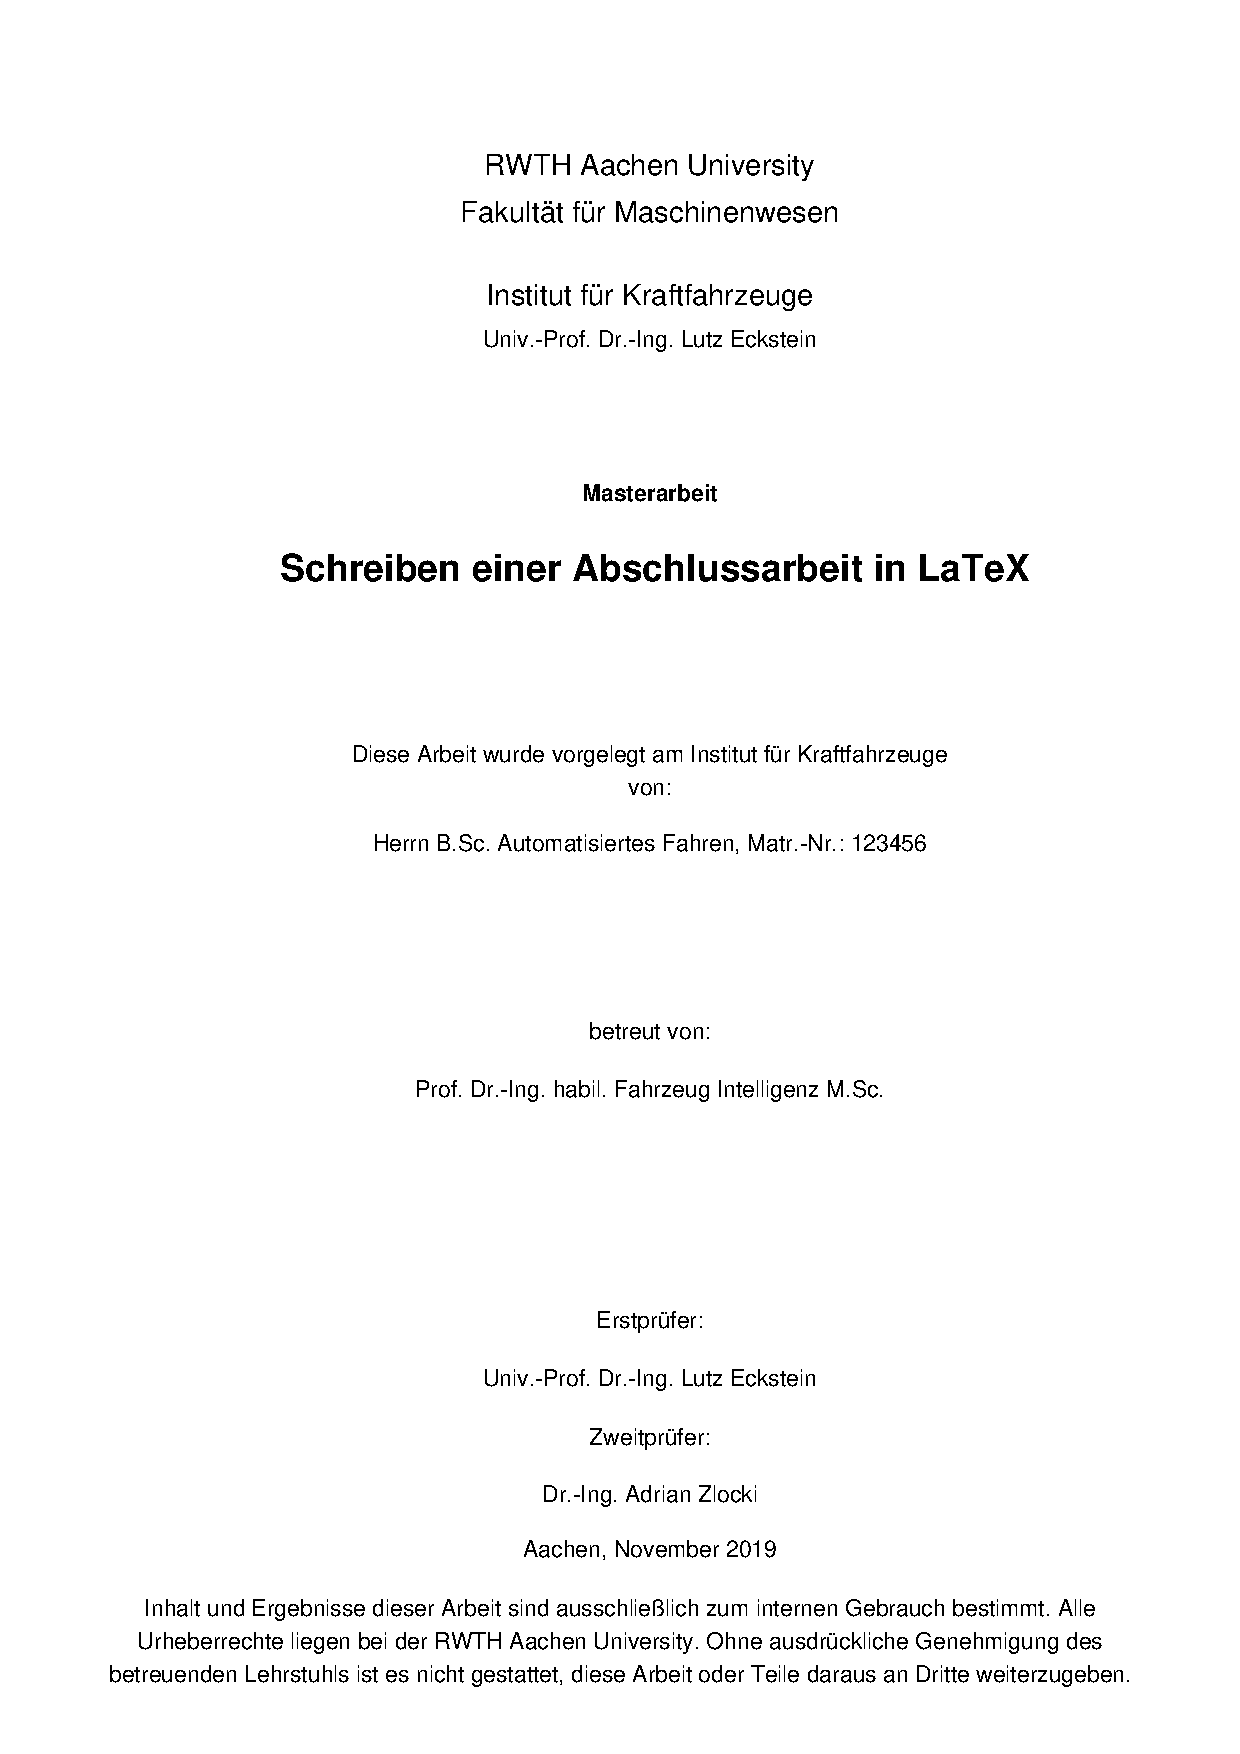
\includepdf[pages={1}]{CoverSheet.pdf}
\newpage

% uncomment for empty page
\thispagestyle{empty}
%\mbox{}
%\newpage
\pagenumbering{arabic}
\pagestyle{plain}
\setcounter{page}{3}
\tableofcontents
\newpage

\pagestyle{ika}

%figures path
\graphicspath{ {./figures/} }

% !TeX root = ../main.tex
\chapter{Introduction}

Nostrud proident anim aliquip et culpa officia ullamco excepteur sint anim commodo.
Veniam in dolore labore aliquip sunt elit voluptate sit. 
Officia eiusmod quis commodo reprehenderit dolore labore aute ea tempor esse ex. 
Pariatur deserunt Lorem excepteur est officia proident magna pariatur adipisicing reprehenderit ex ea ea nulla.

In aliqua elit mollit \gls{cc} est sit aliquip fugiat proident excepteur in irure qui irure anim. 
Voluptate fugiat ut voluptate incididunt qui culpa ea exercitation velit ea ex ad id est. 
Velit exercitation magna ipsum ullamco et laborum do ea consequat.

Reprehenderit amet sunt est quis excepteur labore velit dolor esse veniam dolore eu excepteur velit. 
Amet nisi enim in ullamco in et pariatur duis in deserunt. 
Non proident excepteur labore eu ipsum sunt elit aliquip eu duis incididunt sit laboris. 
Fugiat deserunt do nulla deserunt irure deserunt non proident eu fugiat dolore sint.

Est magna irure amet mollit ullamco. Ex et in cupidatat \glspl{adas} excepteur. 
Reprehenderit sunt incididunt nisi do anim elit aliquip qui officia proident. 
Officia nostrud commodo sit labore cupidatat est irure velit consectetur est est. 
Cupidatat aliqua do in est anim ullamco ullamco enim voluptate ex duis laborum Lorem ad. 
Et minim mollit consequat eiusmod minim ullamco occaecat in proident ex quis. 
Lorem elit commodo eiusmod incididunt quis cupidatat reprehenderit sint irure labore cupidatat quis.

Eiusmod occaecat ex eu enim labore. 
Pariatur ullamco officia duis ea veniam esse consequat sunt do ad sunt. 
Cupidatat adipisicing occaecat nostrud non magna eu exercitation ea laborum veniam sint ullamco et proident.

Aliqua adipisicing elit aliquip laboris mollit voluptate ex incididunt. 
Tempor laboris fugiat proident ut voluptate veniam elit deserunt. 
Quis laborum proident exercitation exercitation aliqua sit pariatur enim aute laborum cupidatat Lorem. 
Reprehenderit fugiat ut sunt culpa ad sunt. Tempor exercitation aliquip tempor aliqua reprehenderit.

% !TeX root = ../main.tex
\chapter{Architecture}
SpatialDETR is the framework chosen for incorporating explainability features, which are visualized using the Application described in Chapter \cite{ch:app}. It is a state-of-the-art 3D Object Detection model based on the Transformer model. Therefore, it is important to understand its architecture and how we can explain its reasoning.
SpatialDETR is actually an extension to the DETR3D architecture, which in turn is based on the popular DETR (DEtection TRansformer). 
In this chapter, DETR is first introduced, which forms the basis of many transformer-based object detection models. Then, DETR3D architecture is described. Finally, SpatialDETR is extensivly described by also highlighting the differences with DETR3D.
\label{ch:sota}
\section{DEtection TRansformer - DETR}
Object detection involves the identification of one or more objects in an image by drawing bounding boxes around them and assigning their labels. It is a more complex task than image classification, which predicts the class of only one object in an image.
DETR is a 2D Object Detector based on an encoder-decoder transformer model, developed by the Facebook AI team \cite{carion2020end}. It is simpler and more accurate than the well-established object detectors such as Faster R-CNN \cite{ren2015faster}. 
The state-of-the-art 2D object detectors are typically two-stage detectors \cite{girshick2015fast} \cite{carion2020end}: they first extract "candidate" regions of object and then they extract features from those regions (by using fully convolutional neural networks) which are finally classified by a fully connected layer. Furthemore, post-processing steps such as NMS (non-maximal suppression) are needed for avoiding near-duplicates

\section{DETR3D}
...

\section{SpatialDETR}
...

\chapter{Explainable Transformer}
Explainability has a well established literature for natural language processing, with techniques such as SHAP and LIME. However, in computer vision there are not standard techniques for explainability. This is even more lacking in for the Transformer architecture. 
However, only in the last years there have been some work toward Explainable Transformer, applied to DeiT and DETR models \cite{touvron2021training} \cite{chefer2021transformer} \cite{chefer2021generic}. Unfortunately, as far as I know there are yet any work toward explaining transformer-based 3D Object Detection.
It is however possible to implement those techniques for SpatialDETR, and even to other 3D object detectors. 
In this chapter, some techniques used for Explainable Transformers are described, such as Attention Rollout and Gradient Rollout. Then, I will discuss how to implement those to the SpatialDETR architecture.  
% !TeX root = ../main.tex
\chapter{Research Questions}
\label{ch:rq}
This thesis should for example help to answer the following questions regarding a multi-sensor 3D Object detector based on a Transformer:
\begin{itemize}
    \item What is happening inside the Transformer on the current input sequence ?
    \item What did the Transformer learn ?
    \item What did the Transformer see in the multi-sensor data stream ?
    \item Where is the Transformer ”looking” at ?
    \item Which sensor(s) is(are) responsible for the current detection ?
  \end{itemize}
% !TeX root = ../main.tex
\chapter{Application Tool}
\label{ch:app}
For addressing the objectives of the thesis, a software application has been developed which helps us to understand the reasoning of the SpatialDETR model. Trying to make it adaptable, a model selection is allowed. Therefore, it is possible to use it for various SpatialDETR configuration, e.g with only query center projection. 
At the moment, the application is addressed to developers who want to see how the 3D Detection works behind the scene. 
It is possible to select the attention visualization mechanism (e.g head fusion, attention rollout, gradient rollout), the attention discard ratio, the  layer (6 in SpatialDETR), the camera (6 in NuScenes dataset). 
Furthemore, it is possible to select the prediction threshold for detection and to visualize the ground trouth bounding boxes. All this flexibility allows for a better understanding of the Transformer model and will help to decide, for example, which attention visualization mechanism better explains the model. 
Therefore this application can be adapted to normal users and authorities by selecting the best configuration for XAI.

% !TeX root = ../main.tex

\chapter{Conclusion \& Outlook}
\label{ch:conclusion}

\pagestyle{plain}


\setlength\LTleft{-6pt}
\setlength\LTright{0pt}

% List of symbols
\printglossary[type=symbolslist,style=symbunitlong,title=List of Symbols,toctitle=Symbols]

% List of Abbreviations
\printglossary[type=acronym,style=long,title=List of Abbreviations,toctitle=Abbreviations]

% Bibliography list
\printbibliography

% Appendix
% !TeX root = ../main.tex
\chapter{Appendix}


\glsaddall

\end{document}